% All figures are inline TikZ; no external EPS conversion is needed.
\newcommand{\DoNotLoadEpstopdf}{}
\documentclass[11pt]{article}
\usepackage[a4paper,margin=27mm]{geometry}
\usepackage{amsmath,amssymb,amsthm,mathtools}
\usepackage{tikz}
\usetikzlibrary{arrows.meta,calc}
\usepackage{flafter}
\usepackage[hidelinks]{hyperref}
\newtheorem{theorem}{Theorem}
\newtheorem{lemma}[theorem]{Lemma}
\newtheorem{proposition}[theorem]{Proposition}
\newtheorem{corollary}[theorem]{Corollary}
\theoremstyle{remark}
\newtheorem{remark}[theorem]{Remark}
\newcommand{\HH}{\mathbb H}
\newcommand{\RR}{\mathbb R}
\newcommand{\ip}[2]{\langle #1,#2\rangle}
\newcommand{\norm}[1]{\lVert #1\rVert}
\newcommand{\CELL}{\mathcal C}

\title{Sharp dimension bounds for right-angled\linebreak hyperbolic polytopes}
\author{Alexander Kolpakov}
\date{28 October 2026}

\begin{document}
\maketitle
\begin{abstract}
We prove that a finite-volume right-angled hyperbolic polytope has
dimension at most eight, and at most four if all its vertices are ideal.
Both bounds are attained. The proofs share an elementary projection:
from a finite interior point, project to a facet of maximum unit-normal
height. Repeating this operation three times in dimension nine gives
a six-face whose wall directions form a spherical code with pairwise
products strictly below $1/4$. A cubic tensor-square identity bounds
this code by $26$, contradicting the published minimum of $27$ facets.
For the ideal bound, one projection in dimension five combines
Musin's kissing-number theorem and Kolpakov's $24$-cell rigidity;
an opposite-normal calculation excludes the metric equality case.
\end{abstract}

\section{Introduction}

Right-angled hyperbolic polytopes provide fundamental domains for
reflection groups, but their possible dimensions have remained separated
from the dimensions of the known constructions. Potyagailo and
Vinberg~\cite{PV} construct finite-volume examples through dimension
eight. Dufour~\cite{Dufour} proves that their dimension is at most
twelve. For polytopes whose vertices are all ideal, the regular
right-angled $24$-cell gives an example in dimension four, whereas
Kolpakov~\cite[Corollary~7]{Kolpakov} obtains the upper bound six.
We close these two gaps. The compact case already has the sharp
dimension bound four; see~\cite[Section~2]{PV}.

A polytope is \emph{entirely ideal} if all its vertices are ideal.
Throughout, hyperbolic polytopes have finitely many facets and finite
volume, and the curvature is normalized to $-1$.
A right-angled polytope has dihedral angle $\pi/2$ at every
actual ridge. Finite and ideal vertices are otherwise allowed in any
combination, and no arithmetic hypothesis is imposed.

\begin{theorem}[All vertex types]\label{thm:general}
A finite-volume right-angled hyperbolic polytope has dimension at
most eight.
\end{theorem}

\begin{theorem}[Entirely ideal polytopes]\label{thm:ideal}
An entirely ideal finite-volume right-angled hyperbolic polytope has
dimension at most four.
\end{theorem}

Finite-volume right-angled examples in dimension eight are recalled
in~\cite{PV}. The regular ideal right-angled $24$-cell gives the
four-dimensional example. Thus both bounds are sharp.

\subsection{Outline of the proofs}
Both arguments begin with the same geometric observation. Projecting
a finite interior point to a facet of maximum unit-normal height
gives an interior point of that facet and decreases every inherited
height by a controlled factor. Repetition produces a low-dimensional
face whose outward normals determine a small spherical code.

For Theorem~\ref{thm:general}, three projections in dimension nine
give a six-face. An explicit cubic sum of tensor squares then bounds
its number of facets by $26$, contradicting the known minimum $27$.
For Theorem~\ref{thm:ideal}, one projection in dimension five gives
an ideal four-dimensional facet with at most $24$ facets. The
minimum-facet theorem identifies it with the regular $24$-cell, and
its opposite wall normals contradict the strict height bound.
The projection is proved in Section~\ref{sec:descent}; the two
contradictions follow in Sections~\ref{sec:code} and~\ref{sec:ideal}.
Figures~\ref{fig:ladder} and~\ref{fig:idealbranch} summarize the two
reductions. All algebra needed for these deductions is displayed in
the paper.

\subsection{Published geometric inputs}
We use the following three numerical statements with their indicated
scopes.

\begin{proposition}[Six-dimensional facet minimum]\label{prop:27}
A six-dimensional finite-volume right-angled hyperbolic polytope
has at least $27$ facets.
\end{proposition}

This is the consequence of Lemma~1 and Proposition~4 of
Dufour~\cite{Dufour} explicitly recalled in~\cite[Section~4]{Alex}.
It applies to every vertex type, rather than only entirely ideal
polytopes. We need neither a classification nor an equality statement
for $27$ facets.

\begin{proposition}[Musin]\label{prop:musin}
A finite subset of $S^3\subset\RR^4$ with pairwise products at most
$1/2$ between distinct members has cardinality at most $24$.
\end{proposition}

This is the Main theorem of~\cite[p.~4]{Musin}. We use its
cardinality bound, not uniqueness of a kissing configuration.

\begin{proposition}[Kolpakov]\label{prop:24}
An entirely ideal right-angled hyperbolic four-polytope has at least
$24$ facets. Equality holds only for the regular ideal right-angled
$24$-cell, up to hyperbolic isometry.
\end{proposition}

This is Theorem~4 of the published paper~\cite[p.~1945]{Kolpakov}.
The last two propositions are needed only for Theorem~\ref{thm:ideal}.
The spherical bound used for Theorem~\ref{thm:general} is proved
directly in Section~\ref{sec:code}.

We use standard geometric foundations for acute-angled polytopes.
In the Lorentz model, distinct outward unit facet normals have
nonpositive products, including facets that do not share a ridge.
As explained in~\cite[p.~42, \S2.1]{Vinberg}, actual nonobtuse ridge
angles imply the all-wall condition: nonadjacent supporting planes
do not intersect, and the off-diagonal Gram entries are nonpositive.
Faces of dimension at least three inherit right angles: every
intrinsic ridge has a finite relative-interior point, where the
incident walls are orthogonal. In the Klein closure, a face has
vertices among those of the original polytope, so entire ideality is
inherited. Triangulation into finite or ideal simplices gives finite
volume. No projection chain below reaches a two-face, where ideal
polygon angles would require separate treatment.

\section{Descending maximum facet height}\label{sec:descent}

Use Lorentz signature $(-,+,\ldots,+)$, future unit timelike points,
and outward \emph{unit} spacelike normals. Thus
\[
 P=\{x\in\HH^n:\ip{x}{m}\le0\text{ for every actual facet normal }m\},
 \qquad \ip{m}{m'}\le0\quad(m\ne m').
\]
All heights below refer to this fixed unit-normal scaling. They are
the hyperbolic sines of distances to the corresponding walls.

\begin{lemma}[Farthest-facet projection]\label{lem:projection}
Let $q$ be a finite relative-interior point of a right-angled polytope
$P$, with $q^2=-1$. Set $t(m)=-\ip{q}{m}>0$, choose a facet normal
$n$ with largest height $t=t(n)$, and put
\begin{equation}\label{eq:projection}
 q'=\frac{q+tn}{\sqrt{1+t^2}}.
\end{equation}
Then $q'$ lies in the relative interior of the actual facet
$Q=P\cap n^\perp$. Every intrinsic facet normal $m_i$ of $Q$ is
an actual ridge neighbor of $n$, remains unit, and has height
\begin{equation}\label{eq:newheight}
 0<t'_i=-\ip{q'}{m_i}
       =\frac{t(m_i)}{\sqrt{1+t^2}}
       \le\frac{t}{\sqrt{1+t^2}}<1.
\end{equation}
\end{lemma}
\begin{proof}
The numerator in~\eqref{eq:projection} has square $-1-t^2$ and
product zero with $n$. Its product with $q$ is $-1-t^2<0$, so
normalization gives a future unit point in $n^\perp$. For \emph{any}
other actual facet normal $m$,
\begin{equation}\label{eq:allwall}
 \ip{q'}{m}=\frac{\ip{q}{m}+t\ip{n}{m}}{\sqrt{1+t^2}}<0.
\end{equation}
The first numerator term is strict and the second is nonpositive.
Thus $q'$ lies in the actual facet and is strict against all other
walls; it is not merely a formal point on the supporting plane.

An intrinsic facet of $Q$ comes from its unique ridge neighbor $m_i$.
Right angles give $\ip{n}{m_i}=0$, so restriction to $n^\perp$
preserves its unit norm. Formula~\eqref{eq:newheight} now follows
from the maximum choice of $t$.
\end{proof}

If all heights at $q$ are at most $A$, monotonicity of
$x/\sqrt{1+x^2}$ gives a new bound
$A/\sqrt{1+A^2}$. Start with the finite maximum $A_0$ at any finite
interior point, and let $A_j$ be the maximum height after $j$
projections. Repeating the construction intrinsically gives
\begin{equation}\label{eq:iterate}
 A_j\le\frac{A_0}{\sqrt{1+jA_0^2}}<\frac1{\sqrt j}
 \qquad(j\ge1),
\end{equation}
whenever the selected faces still have dimension at least three.
The formula follows by induction, or by adding one to the inverse
square of the previous bound. Strictness holds even if the maximizing
facet is not unique at a step.

\begin{figure}[t]
\centering
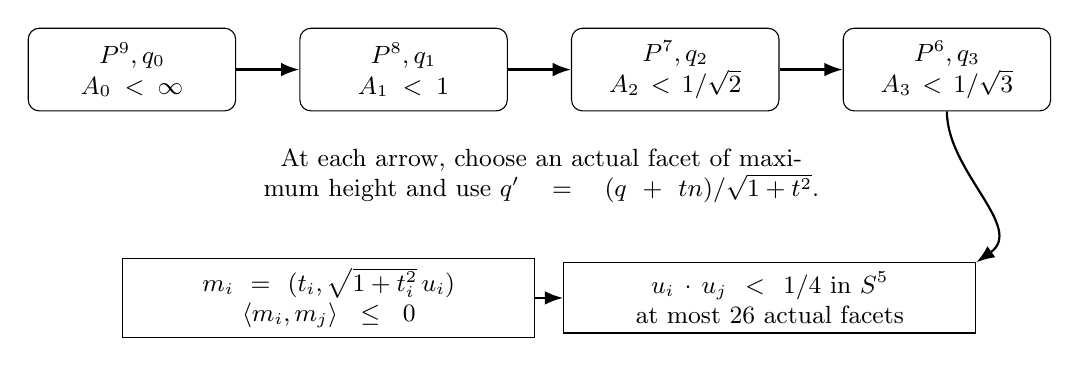
\begin{tikzpicture}[>=Latex,font=\small,
 box/.style={draw,rounded corners,align=center,text width=2.4cm,
             minimum height=1.05cm}]
 \node[box] (q0) at(0,1.4) {$P^9,q_0$\\$A_0<\infty$};
 \node[box] (q1) at(3.45,1.4) {$P^8,q_1$\\$A_1<1$};
 \node[box] (q2) at(6.9,1.4) {$P^7,q_2$\\$A_2<1/\sqrt2$};
 \node[box] (q3) at(10.35,1.4) {$P^6,q_3$\\$A_3<1/\sqrt3$};
 \draw[->,thick] (q0)--(q1);
 \draw[->,thick] (q1)--(q2);
 \draw[->,thick] (q2)--(q3);
 \node[align=center,text width=11.7cm] at(5.2,.05)
  {At each arrow, choose an actual facet of maximum height and use
   $q'=(q+tn)/\sqrt{1+t^2}$.};
 \node[draw,align=center,text width=5cm] (split) at(2.5,-1.5)
  {$m_i=(t_i,\sqrt{1+t_i^2}\,u_i)$\\
   $\ip{m_i}{m_j}\le0$};
 \node[draw,align=center,text width=5cm] (code) at(8.1,-1.5)
  {$u_i\cdot u_j<1/4$ in $S^5$\\
   at most $26$ actual facets};
 \draw[->,thick] (q3.south) to[out=-90,in=35] (code.north east);
 \draw[->,thick] (split)--(code);
\end{tikzpicture}
\caption{Three actual facet choices and the resulting spherical code.
The arrows are the exact projection formulas, not ordinary edges of
the polytope. The final code has one direction for each actual facet;
the tensor calculation below contradicts the published minimum of $27$.}
\label{fig:ladder}
\end{figure}

We will use the following translation from heights to spherical codes.
At a unit point $q$ of a $d$-dimensional face, choose $q$ as its time
axis and write the intrinsic unit normals as
\begin{equation}\label{eq:split}
 m_i=\bigl(t_i,\sqrt{1+t_i^2}\,u_i\bigr),
 \qquad u_i\in S^{d-1}\subset\RR^d.
\end{equation}
For distinct facets, all-wall acuteness gives
\begin{equation}\label{eq:spatial}
 u_i\cdot u_j\le
 \frac{t_it_j}{\sqrt{(1+t_i^2)(1+t_j^2)}}.
\end{equation}
The directions are distinct: if $u_i=u_j$, the Lorentz product of
the two unit normals would be positive. Consequently the number of
code points is exactly the number of facets of the selected face.

\section{A strict spherical bound in six variables}\label{sec:code}

\begin{lemma}\label{lem:26}
A finite set of unit vectors in $\RR^6$ whose distinct-pair products
are strictly less than $1/4$ has at most $26$ members.
\end{lemma}
\begin{proof}
Consider the cubic polynomial
\begin{equation}\label{eq:polynomial}
 F(x)=(x+\tfrac12)^2(x-\tfrac14)
     =x^3+\tfrac34x^2-\tfrac1{16}.
\end{equation}
We give a direct tensor-square proof of the required positive-kernel
identity, so no spherical linear-programming theorem is needed.

Use ordinary Euclidean tensor inner products. For a unit vector $u$
define the rank-two tensor
\[
 A(u)=u\otimes u-I/6
\]
and the symmetric rank-three tensors
\[
 S(u)_{abc}=u_a\delta_{bc}+u_b\delta_{ac}+u_c\delta_{ab},
 \qquad T(u)=u^{\otimes3}-S(u)/8.
\]
For $x=u\cdot v$, contraction gives
\begin{equation}\label{eq:kernels}
 \ip{A(u)}{A(v)}=x^2-\tfrac16,
 \qquad \ip{T(u)}{T(v)}=x^3-\tfrac38x.
\end{equation}
Each cross contraction of a cubic tensor with $S$ is $3x$; the
remaining contraction is
\[
 \ip{S(u)}{S(v)}=(3\cdot6+6)x=24x.
\]
The scalar identity therefore becomes
\begin{align*}
 F(u\cdot v)&=\tfrac1{16}+\tfrac38(u\cdot v)\\
 &\quad+\tfrac34\ip{A(u)}{A(v)}+\ip{T(u)}{T(v)}.
\end{align*}
Thus, for $u_1,\ldots,u_N$,
\begin{align}
 \sum_{i,j}F(u_i\cdot u_j)
 &=\frac{N^2}{16}+\frac38\norm{\sum_i u_i}^2\notag\\
 &\quad+\frac34\norm{\sum_i A(u_i)}^2
   +\norm{\sum_i T(u_i)}^2\notag\\
 &\ge\frac{N^2}{16}.\label{eq:sos}
\end{align}

On the other hand, $F(1)=27/16$, and $F(x)\le0$ for $x<1/4$.
The diagonal terms and~\eqref{eq:sos} give
\[
 \frac{N^2}{16}\le\sum_{i,j}F(u_i\cdot u_j)\le\frac{27N}{16},
\]
so $N\le27$. If $N=27$, equality throughout forces each
off-diagonal polynomial value to vanish. Since $u_i\cdot u_j<1/4$
strictly, the only available root is $-1/2$. Four such vectors would
already give
\[
 \norm{u_1+u_2+u_3+u_4}^2=4+12(-\tfrac12)=-2,
\]
which is impossible. Hence $N\le26$.
\end{proof}

\begin{proof}[Proof of Theorem~\ref{thm:general}]
Suppose first that a right-angled nine-polytope exists. Three
projections from a finite interior point produce an actual six-face
$R$ and a relative-interior point at which every facet height is
strictly less than $1/\sqrt3$, by~\eqref{eq:iterate}.
The inherited face is right-angled and has finite volume.
For its intrinsic normals,~\eqref{eq:spatial} now gives
\[
 u_i\cdot u_j<\frac14\qquad(i\ne j)
\]
in $S^5\subset\RR^6$. Lemma~\ref{lem:26} gives at most $26$
facets for $R$, contradicting Proposition~\ref{prop:27}.
Every higher-dimensional polytope has a nine-face inheriting finite
volume and right angles, giving the same contradiction.
\end{proof}

\section{The ideal bound from one projection}\label{sec:ideal}

We first record the small metric calculation needed at equality.
In the standard Lorentz model of the regular ideal right-angled
$24$-cell, its outward unit normals are
\begin{equation}\label{eq:24normals}
 (1,\epsilon e_i+\delta e_j),\qquad
 1\le i<j\le4,\quad\epsilon,\delta\in\{1,-1\},
\end{equation}
and the center is $(1,0)$.

\begin{lemma}\label{lem:center}
No future unit timelike point of the regular ideal right-angled
$24$-cell has all its unit-normal heights strictly less than one.
More precisely, if every height is at most one, the point is the
center and all the heights equal one.
\end{lemma}
\begin{proof}
The normals in~\eqref{eq:24normals} come in opposite spatial pairs
$(1,r),(1,-r)$. Write the point as $(a,w)$, with $a>0$ and
$a^2-\norm w^2=1$. The two corresponding heights are
$a-r\cdot w$ and $a+r\cdot w$. If both are at most one, their
sum gives $a\le1$. Future unit timelikeness gives $a\ge1$.
Thus $a=1,w=0$, and every height equals one. Strict inequalities
on all heights are impossible.
\end{proof}

\begin{figure}[t]
\centering
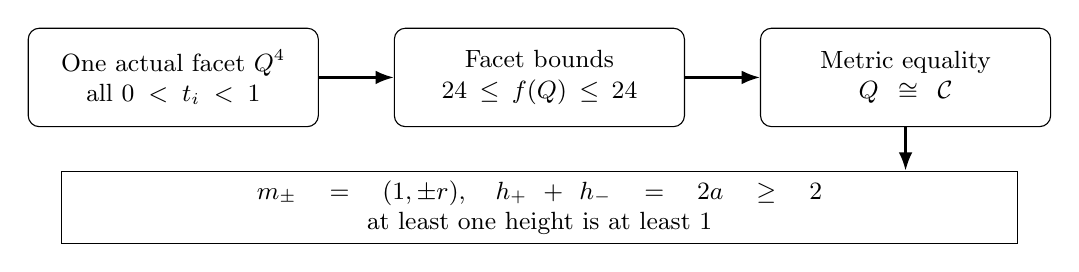
\begin{tikzpicture}[>=Latex,font=\small,
 box/.style={draw,rounded corners,align=center,text width=3.45cm,
             minimum height=1.25cm}]
 \node[box] (facet) at(0,0)
  {One actual facet $Q^4$\\all $0<t_i<1$};
 \node[box] (count) at(4.65,0)
  {Facet bounds\\$24\le f(Q)\le24$};
 \node[box] (metric) at(9.3,0)
  {Metric equality\\$Q\cong\CELL$};
 \draw[->,thick] (facet)--(count);
 \draw[->,thick] (count)--(metric);
 \node[draw,align=center,text width=11.9cm] (pair) at(4.65,-1.65)
  {$m_\pm=(1,\pm r),\quad h_++h_-=2a\ge2$\\
   at least one height is at least $1$};
 \draw[->,thick] (metric.south)--(metric.south |- pair.north);
\end{tikzpicture}
\caption{The ideal branch. Musin's spherical bound and Kolpakov's
facet theorem force metric equality with the regular $24$-cell.
One opposite pair of its wall normals then contradicts the strict
height bound produced by the projection. No uniqueness theorem for
spherical kissing configurations is used.}
\label{fig:idealbranch}
\end{figure}

\begin{proof}[Proof of Theorem~\ref{thm:ideal}]
Assume an entirely ideal right-angled five-polytope exists. A single
farthest-facet projection from a finite interior point gives a
four-dimensional facet $Q$ at whose relative-interior point all heights satisfy
$0<t_i<1$. It inherits finite volume, entire ideality and right angles.
By~\eqref{eq:spatial}, its spherical directions in $S^3$ have
pairwise products strictly below $1/2$. Proposition~\ref{prop:musin}
bounds its facet number by $24$; Proposition~\ref{prop:24} gives the
reverse bound and identifies $Q$ with the regular ideal $24$-cell.
Its metric equality case, not a uniqueness assertion for kissing
configurations, is what is used here. Lemma~\ref{lem:center}
contradicts the strict heights $t_i<1$.

There is no entirely ideal right-angled five-polytope. In any higher
dimension a five-face would inherit all three hypotheses and give
the same contradiction. The ideal right-angled $24$-cell attains
dimension four.
\end{proof}

Both proofs use actual facets and a finite point checked against
every wall. Neither infers a polytope from a set of formal Gram
vectors, nor infers finite volume from a few feasible vertices.
The strict inequalities come from projecting a finite point;
they require no limiting or generic-position argument. For the
general bound the only numerical geometric input is the
six-dimensional facet minimum. For the ideal bound the additional
inputs are exactly Musin's cardinality theorem and Kolpakov's metric
equality theorem. All remaining calculations are displayed above.

\section{Reproducibility and verification scope}\label{sec:reproduce}

The proofs above consist of geometric arguments and the displayed
tensor identities, with the published inputs stated in Section~1.
Accompanying exact Python checks, selected Lean~4 modules and their
execution records are available in the
\href{https://github.com/sashakolpakov/CoxeterPolytopes/tree/04c9bab7}{repository snapshot \texttt{04c9bab7}}.
The catalogue entry for this paper is
\texttt{right\_angled\_sharp}. Its two exact checks have the following
precise purposes.

The \href{https://github.com/sashakolpakov/CoxeterPolytopes/blob/04c9bab7/scripts/check_ideal_right_angled_dimension4_model_20261020.py}{coordinate check}
verifies the $24$ normals in~\eqref{eq:24normals},
their $276$ unordered Gram products, the $12$ opposite pairs and
the displayed null vertices and cubical cusp links. This is a check
of the specified model. The \href{https://github.com/sashakolpakov/CoxeterPolytopes/blob/04c9bab7/scripts/check_right_angled_sharp_dimension_sos_20261020.py}{tensor check}
expands the $36$ rank-two
and $216$ rank-three entries over the rational polynomial ring in
twelve independent variables. It verifies~\eqref{eq:kernels} and
the sum-of-squares identity~\eqref{eq:sos}, including the explicit
remainders modulo the two unit-sphere equations. It also checks the
ratio $27$ and the strict endpoint calculation. These are exact
identities; neither a numerical sample nor an enumeration of
hyperbolic polytopes is involved.

From the repository root, inspect the selected jobs without starting
a proof check:
\begingroup\small
\begin{verbatim}
python3 -B scripts/run_proof_batch_20261024.py manuscript \
  right_angled_sharp --mode scripts --plan
\end{verbatim}
\endgroup
To execute the two checks and retain a receipt, choose a previously
unused ledger filename:
\begingroup\small
\begin{verbatim}
python3 -B scripts/run_proof_batch_20261024.py manuscript \
  right_angled_sharp --mode scripts \
  --ledger results/sharp_replay_new.json
\end{verbatim}
\endgroup
The exact checks require Python~3.11 or later. The guarded runner
executes one job at a time with the repository's macOS resource
monitor; the two checker sources use only the Python standard library.
The optional \texttt{--mode core} selection additionally checks
conditional Lean kernels for projection, the cubic bound and the
dimension implications. The geometric realization, published
theorems and face inheritance remain explicit premises of those
kernels. Their scope is internal logic rather than a complete
formalization of hyperbolic geometry.

The \href{https://github.com/sashakolpakov/CoxeterPolytopes/blob/04c9bab7/docs/right_angled_sharp_dimensions_publication_proof_map_20261021.md}{proof and reproduction guide}
identifies the checker sources and the mathematical statements they
test. The \href{https://github.com/sashakolpakov/CoxeterPolytopes/blob/04c9bab7/docs/right_angled_release_packages_20261025.md}{release guide}
and \href{https://github.com/sashakolpakov/CoxeterPolytopes/blob/04c9bab7/results/right_angled_release_packages_current_20261025.json}{source-bound verification record}
give the exact inputs, saved outcomes and separate formal-verification
boundaries. These records concern their named source editions.
The catalogue's PDF option builds its preserved publication edition;
the present submission adds exposition and reproduction links while
retaining the mathematical argument. Its \texttt{main.tex} is a
standalone source: all figures are inline TikZ and the bibliography
is included below.

\section*{Acknowledgments}
The author used OpenAI's GPT-6-astra and GPT-6.1-sol as research and coding
assistants to investigate proof ideas, help strengthen the results, improve
the exposition, and generate and audit the Python and Lean~4 code
accompanying this paper. The author reviewed the resulting mathematics
and code and takes responsibility for the final content.

\begin{thebibliography}{9}
\raggedright
\bibitem{Alex}
S. Alexandrov, \emph{On ideal vertices of right-angled hyperbolic
polyhedra}, 2023, \href{https://arxiv.org/abs/2303.09533}{arXiv:2303.09533}.

\bibitem{Dufour}
G. Dufour, \emph{Notes on right-angled Coxeter polyhedra in hyperbolic
spaces}, Geometriae Dedicata \textbf{147} (2010), 277--282.
\href{https://doi.org/10.1007/s10711-009-9454-2}{doi:10.1007/s10711-009-9454-2}.

\bibitem{Kolpakov}
A. Kolpakov, \emph{On the optimality of the ideal right-angled
$24$-cell}, Algebraic \& Geometric Topology \textbf{12} (2012),
1941--1960.
\href{https://doi.org/10.2140/agt.2012.12.1941}{doi:10.2140/agt.2012.12.1941}.

\bibitem{Musin}
O. R. Musin, \emph{The kissing number in four dimensions}, Annals of
Mathematics (2) \textbf{168} (2008), 1--32.
\href{https://doi.org/10.4007/annals.2008.168.1}{doi:10.4007/annals.2008.168.1}.

\bibitem{PV}
L. Potyagailo and E. B. Vinberg, \emph{On right-angled reflection
groups in hyperbolic spaces}, Commentarii Mathematici Helvetici
\textbf{80} (2005), 63--73.
\href{https://doi.org/10.4171/CMH/4}{doi:10.4171/CMH/4}.

\bibitem{Vinberg}
E. B. Vinberg, \emph{Hyperbolic reflection groups}, Russian Mathematical
Surveys \textbf{40}:1 (1985), 31--75.
\href{https://doi.org/10.1070/RM1985v040n01ABEH003527}{doi:10.1070/RM1985v040n01ABEH003527}.
\end{thebibliography}
\end{document}
